\chapter{Scenarios}

The practical part of this tutorial is built around realistic scenarios that introduce various aspects of \SES, ranging from basic the input to the implementation of 3D models, the compuation of sensitivity kernels, and rotations of the computational domain. For each of the scenarios, various source and input files must be changed. Those files can be found in the \texttt{SCENARIOS} folder.

%====================================================================
% Anatolia
%====================================================================

\section{Regional-scale wave propagation: Anatolia}\label{S:Anatolia}

In our first scenario, we work with an earthquake that occurred on August 25, 2007 in eastern Turkey. The hypocentre location is: latitude: $39.26^\circ$, longitude: $41.04^\circ$, depth: $5.0$ km. Our goal is to introduce the input files of \SES, implement a 3D heterogeneous model, and compute sensitivity kernels.\\[5pt]
The default setup of \SES is made to fully reproduce this example. All input and source files that are specific to this scenario can also be found in the \texttt{SCENARIOS/ANATOLIA/} folder.

%- Input ===============================================================

\subsection{Input}

\subsubsection{Model setup}\label{S:model_setup}

The geometrical setup of the model is described in the file \texttt{setup} in the directory \texttt{INPUT}. In our specific example, the computational domain ranges from $47.1^\circ - 55.9^\circ$ colatitude (colatitude$=90^\circ -$latitude), from $23.1^\circ - 42.9^\circ$ longitude, and from a radius of $5,900,000.0 - 6,371,000.0$ m, i.e. from $471$ km depth to the surface of the Earth. For the moment, we ignore visco-elastic dissipation (\texttt{is\_diss=0}), and we construct a homogeneous model where all velocities and density are set to zero (\texttt{model\_type=1}). More on the generation of specific Earth models can be found in section \ref{S:model_generation}.\\[5pt]
We parallelise the computations by dividing the computational domain into $3$ subdomains in colatitudinal direction (\texttt{px}=3), $4$ subdomains in longitudinal direction (\texttt{py}=4) and $4$ subdomains in depth direction (\texttt{pz}=4). Thus, we have a total of $48$ subdomains, each of which is assigned to one compute core. The parallelisation in \SES is shown schematically in figure \ref{F:parallel}.\\[5pt]
Within each of the subdomains, the finite elements are numbered from $0$ to $66$/\texttt{px}$=22$ in colatitudinal direction (\texttt{nx\_global=66}), from $0$ to $108$/\texttt{py}$=27$ in longitudinal direction (\texttt{ny\_global=108}), and from $0$ to $28$/\texttt{pz}$=7$ in radial direction (\texttt{nz\_global=28}). The total number of elements in the complete computational domain is (\texttt{nx\_global}+\texttt{px})(\texttt{ny\_global}+\texttt{py})(\texttt{nz\_global}+\texttt{pz})$=247,296$. Note that the ratios\\[5pt]
\texttt{nx\_max}=\texttt{nx\_global}/\texttt{px}, \texttt{ny\_max}=\texttt{ny\_global}/\texttt{py} and \texttt{nz\_max}=\texttt{nz\_global}/\texttt{pz}\\[5pt]
must all be integers. The values of \texttt{nx\_max}, \texttt{ny\_max} and \texttt{nz\_max} must be set in the first lines of the source file \texttt{ses3d\_modules.f90} in the directory \texttt{SOURCE}, \textbf{and the code must be recompiled after changing these numbers.}\\[5pt]
Within each element, the dynamic fields (e.g. stress tensor, displacement field, ...) are represented by Lagrange polynomials of degree $4$ (\texttt{lpd}=4). One element therefore comprises $(4+1)^3=125$ grid points, meaning that the complete computational domain contains $247,296 \cdot 125 = 30,912,000$ grid points.\\[5pt]
For the moment, we perform a pure forward simulation, and therefore set the parameter \texttt{adjoint\_flag} to $0$. The remaining parameters in the \texttt{setup} file, as well as the actual meaning of the  \texttt{adjoint\_flag} will be discussed in section \ref{S:kernels}.
%====================================================================
\begin{center}
\begin{figure}
\center\scalebox{0.37}{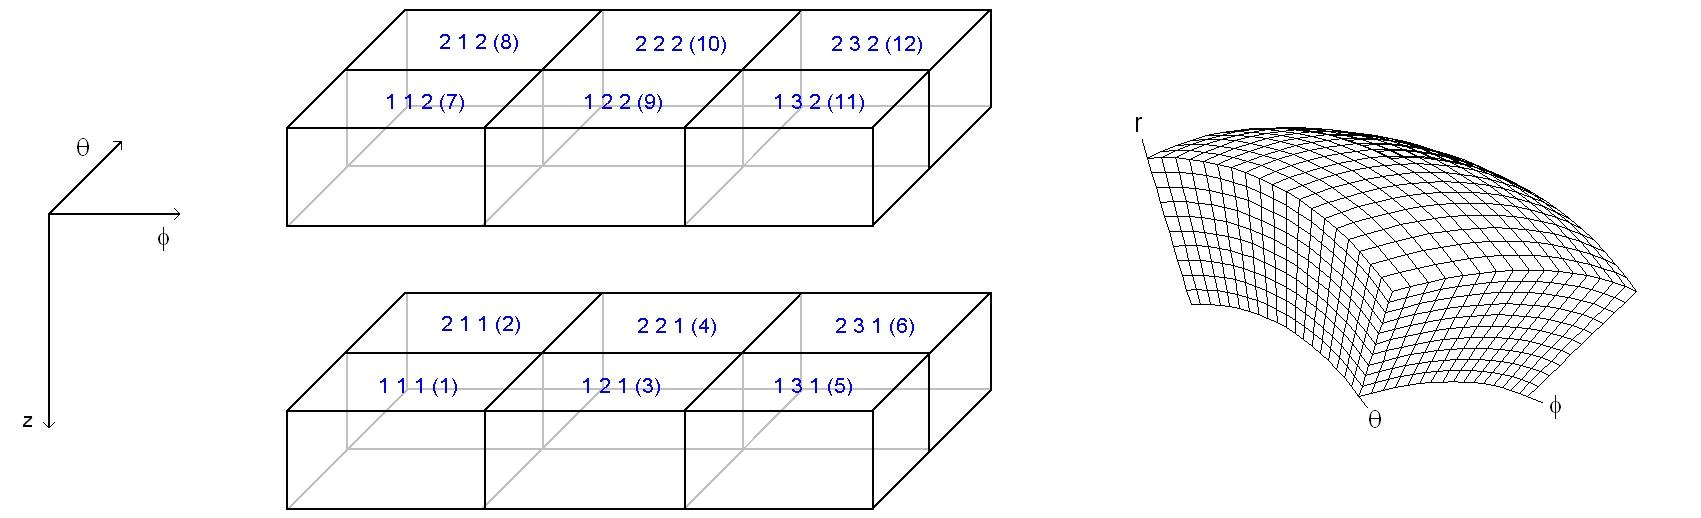
\includegraphics{Figures/parallel_boxes.jpg}} 
\caption{Schematic representation of the parallelisation of \SES. The spherical section is subdivided into subsections, and each subsection is assigned to one compute core. A triple index and a single index (in parenthesis) is assigned to a subsection.}\label{F:parallel}
\end{figure}
\end{center}
%====================================================================

\subsubsection{Event information}

\SES can model a sequence of earthquakes (events), each labelled by an integer number. The event information for the event numbered $x$ is contained in the file \texttt{event\_x}. A list of all events to be modelled must be provided in the file \texttt{event\_list} (number of events followed by their label).\\[5pt]
In this example, we label our event with $1$. The event information in the file \texttt{event\_1} are the colatitude (\texttt{xxs}$=50.740^\circ$), longitude (\texttt{yys}$=41.040^\circ$) and depth (\texttt{zzs}$=5,000$ m) of the source. The source type (\texttt{srctype}) is set to $3$, which indicates a moment tensor source. (The options \texttt{srctype}=$1,2,3$ correspond to vector forces in the colatitudinal, longitudinal and radial directions, respectively.) The moment tensor in our simulation corresponds to an explosion:
\begin{equation}
\w{M}=\begin{pmatrix}
M_{\theta\theta} & M_{\theta\phi} & M_{\theta r} \\
M_{\theta\phi} & M_{\phi\phi} & M_{\phi r} \\
M_{\theta r} & M_{\phi r} & M_{ r r}
\end{pmatrix}
=
\begin{pmatrix}
1.0 & 0.0 & 0.0 \\
0.0 & 1.0 & 0.0 \\
0.0 & 0.0 & 1.0
\end{pmatrix}\, \cdot 10^{16}\,\text{N\,m}\,.
\end{equation}
In our simulation we perform \texttt{nt}$=4,000$ time steps, each of which is \texttt{dt}$=0.13$ s long. As output directory for the synthetic seismograms we set \texttt{../DATA/OUTPUT/1.8s/}.

\subsubsection{Receiver locations}

A list of receivers must be provided in the file \texttt{recfile\_*} located in the \texttt{INPUT} directory. The * is to be replaced by the event number, i.e. we have \texttt{recfile\_1} in our case. Following the number of receivers in the list, each receiver is listed with its name and, in the line below, colatitude ($^\circ$), longitude ($^\circ$) and depth (m). The depth must be larger or equal to zero, i.e., no receivers are allowed above the surface. Each receiver name is exactly $12$ characters long. These characters are typically occupied by the actual station name, the network and any type of additional information.

\subsubsection{Source time function}

The source time function \texttt{stf} is given in the \texttt{INPUT} directory in the form of an ASCII list. Each entry is a sample of the source time function, and the time spacing must equal the one in the \texttt{event\_*} files. (This time spacing is not given explicity in \texttt{stf}. In our case it is \texttt{dt}$=0.13$ s.)\\[5pt]
The source time function should ideally be a bandpass filtered Heaviside function. Periods that are too long cannot be modelled because the computational domain is finite, and periods that are too short cannot be modelled accurately because of discretisation errors. (Furthermore, short periods tend to produce artefacts when they interact with the absorbing boundaries.) As a rule of thumb, the shortest period in the source time function should be such that the corresponding wavelength is not shorter than $1.5$ to $2$ elements. In our case, one element is around $14$ km wide (e.g. $69$ elements over a distance of $55.9^\circ-47.1^\circ=8.8^\circ$), meaning that the minimum wavelength should be $21$ to $28$ km. Assuming a minimum propagation velocity of around $3$ km$/$s, this translates to a minimum period of $7$ to $9$ s. For our example we use a Heaviside function filtered between $8$ s and $100$ s (see figure \ref{F:stf}).
%====================================================================
\begin{center}
\begin{figure}
\center\scalebox{0.30}{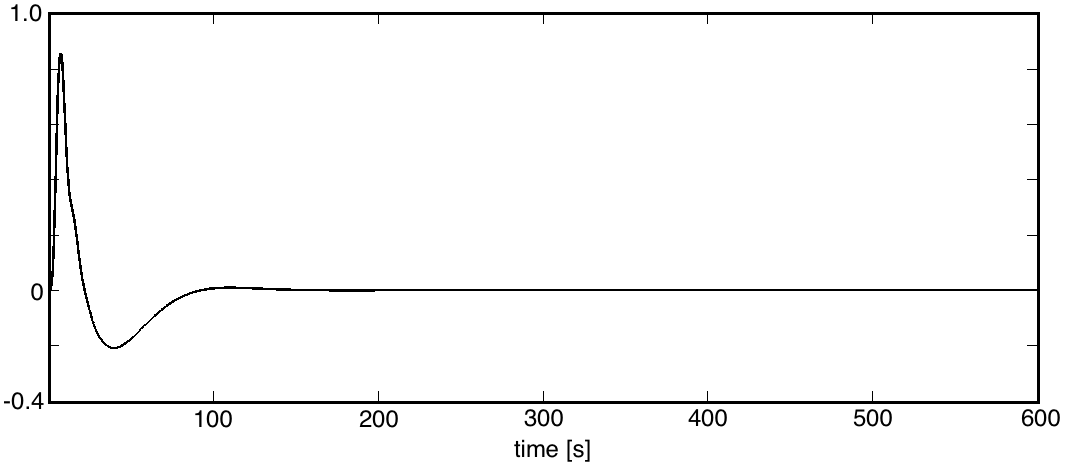
\includegraphics{Figures/stf.png}} 
\caption{Source time function. We use a Heaviside function bandpass filtered between $8$ s and $100$ s. The number of samples in the source time function file \texttt{stf} must be at least the number of time steps \texttt{nt} given in the event files \texttt{event\_*}.}\label{F:stf}
\end{figure}
\end{center}
%====================================================================


%====================================================================
% Model generation
%====================================================================

\subsection{Model construction}\label{S:model_generation}

The construction of 3D Earth models in \SES is proceeds in two steps: (1) The construction of a 1D, i.e. radially symmetric, Earth model, and (2) the addition of 3D perturbations to the 1D model. To facilitate the solution of tomographic inverse problems, model construction in \SES is completely decoupled from the actual wave propagation. The necessary executables can be generated by compiling the source code located in \texttt{MODELS/SOURCE}, e.g. by running the script \texttt{s\_make}. The executables are located in \texttt{MODELS/MAIN}.

\subsubsection{Step 1: Constructing 1D Earth models}

We construct 1D Earth models by running \texttt{generate\_models.exe}, located in \texttt{MODELS/MAIN}. This programme reads the geometrical setup provided in the \texttt{setup} file. The type of 1D Earth model is specified by the parameter \texttt{model\_type} in the \texttt{setup} file. In our case, \texttt{model\_type}$=1$, which generates a homogeneous model with all velocities and density set to zero.\\[5pt]
The following alternative Earth models are currently implemented:
\begin{enumerate}
\item \texttt{model\_type=2}: Isotropic version of PREM (Dziewonski and Anderson, 1981).
\item \texttt{model\_type=3}: All-zero elastic model with a smoothed version of the Q model QL6 (Durek \& Ekstr\"{o}m).
\item \texttt{model\_type=4}: Modified version of the isotropic PREM with the 220 km discontinuity replaced by a linear gradient.
\item \texttt{model\_type=7}: AK135 (Kennett et al., 1995).
\end{enumerate}
The detailed setups of these 1D model can be found in \texttt{MODELS/MODELS\_1D}.\\[5pt]
Running \texttt{generate\_models.exe} produces files containing the physical model parameters ($\lambda, \mu, A, B, C$ and $1/\rho$) for each of the computational subdomains ($48$ in our case). These are located in \texttt{MODELS/MODELS}. Furthermore, \texttt{generate\_models.exe} writes the \texttt{boxfile} which summarises the geometrical setup and the parallelisation of the computational domain. All these files serve as input for the actual wave propagation.\\[5pt]
For debugging purposes, \texttt{generate\_models.exe} also writes human-readable vertical profiles through each of the subdomains. These are named \texttt{prof\_*}, where * denotes the index of the subdomain.

\subsubsection{Step 2: Adding 3D heterogeneity}

\paragraph{Description of 3D heterogeneous models}\label{S:3Dmodels}

Following the construction of a 1D model, we add 3D perturbations, located in \texttt{MODELS/MODELS\_3D}. The term \emph{3D perturbations} is loosely defined. In our specific case where the 1D model is the homogeneous model with all parameters set to zero, the perturbations are in fact the absolute 3D model itself.\\[5pt]
The 3D perturbations of P velocity (in km$/$s, file \texttt{dvp}), SH velocity (in km$/$s, file \texttt{dvsh}), SV velocity (in km$/$s, file \texttt{dvsv}) and density (in g$/$cm$^3$, file \texttt{drho}) are parametrised in discrete regular blocks. The geometry of the blocks, i.e. the locations of their bounding grid points, is descibed in the files \texttt{block\_x} (colatitudinal direction), \texttt{block\_y} (longitudinal direction) and \texttt{block\_z} (radial direction).\\[5pt]
In our specific example, the horizontal grid spacing is $0.25^\circ$ from $5871$ km to $6266$ km radius, and $0.1^\circ$ from $6266$ km to $6371$ km radius. The radial grid spacing is $5$ km throughout the model. This variable grid spacing roughly reflects the tomographic resolution that we expect in different depth ranges. Figure \ref{F:block_files} illustrates how the variable grid spacing within the two subdomains is represented in the \texttt{block\_*} files. A schematic representation of the grid spacing is shown in figure \ref{F:geometry}.\\[5pt]
Note that the grid on which the 3D model is described, is completely independent of the numerical grid used in the wave propagation machinery or for the generation of the 1D model. This independence allows us to add 3D model perturbations to any previously constructed 1D model - regardless of its specific setup.\\[5pt]
The files containing the actual model perturbations (\texttt{dvp, dvsh, dvsv, drho}) are organised as shown in figure \ref{F:perturbations}. Note that the velocity and density values are given for the volumetric blocks bounded by the grid points. The number of blocks is therefore smaller than the number of grid points.
%====================================================================
\begin{center}
\begin{figure}
\center\scalebox{0.35}{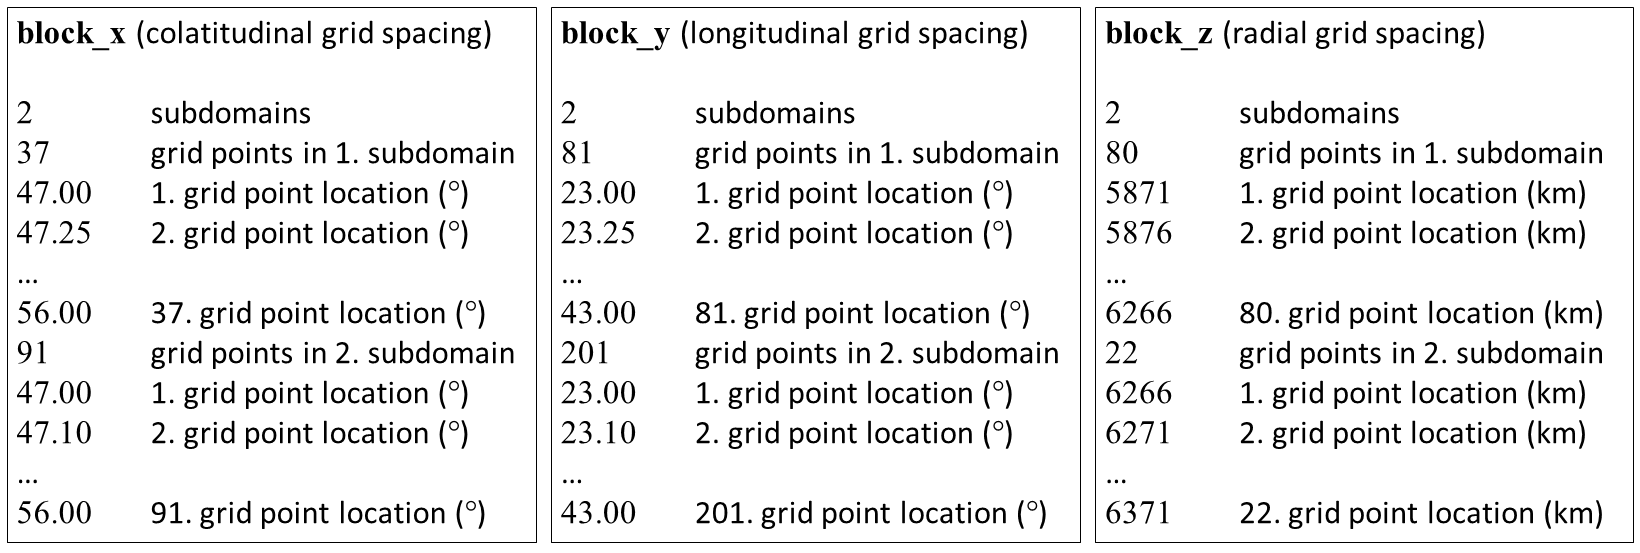
\includegraphics{Figures/block_files.png}} 
\caption{Organisation of the \texttt{block\_*} files that describe the geometric parametrisation of the 3D heterogeneities.}\label{F:block_files}
\end{figure}
\end{center}
%====================================================================
%====================================================================
\begin{center}
\begin{figure}
\center\scalebox{0.35}{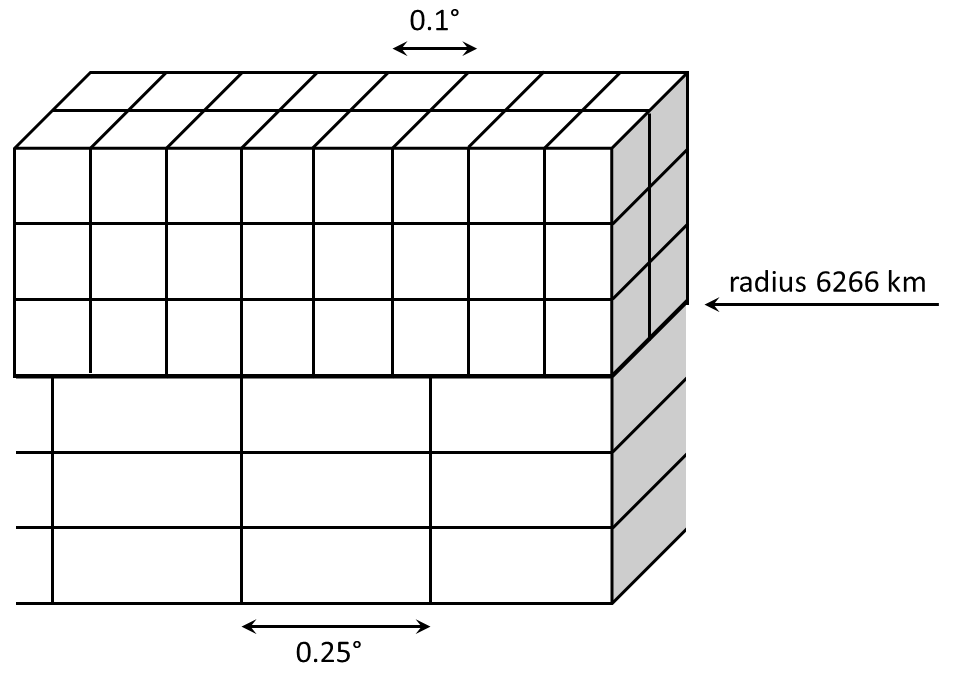
\includegraphics{Figures/geometry.png}} 
\caption{Schematic representation of the variable grid spacing of the 3D heterogeneities. Above a radius of $6266$ km, the horizontal grid spacing is $0.1^\circ$. Below, it is $0.25^\circ$.}\label{F:geometry}
\end{figure}
\end{center}
%====================================================================
%====================================================================
\begin{center}
\begin{figure}
\center\scalebox{0.35}{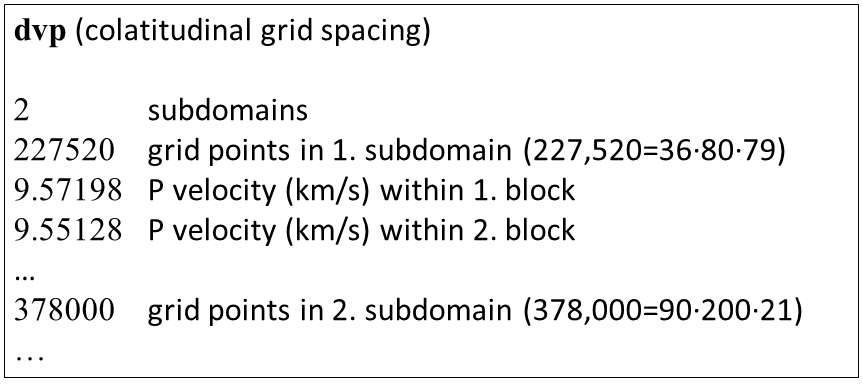
\includegraphics{Figures/perturbations.png}} 
\caption{Organisation of the P velocity perturbations in the file \texttt{dvp}. The number of subdomains ($2$) is followed by the number of blocks in the first subdomain ($227,520$). The actual values of P velocity (perturbations) are given as a list that results from looping over the 3D volume. The outer loop if over colatitude, the intermediate loop over longitude, and the inner loop over radius. This list is then followed by a similar list for the second subvolume. The files \texttt{dvsh}, \texttt{dvsv} and \texttt{drho} are organised analogously.}\label{F:perturbations}
\end{figure}
\end{center}
%====================================================================

\paragraph{Adding 3D heterogeneity to the 1D model}

We can add 3D perturbations in $\vp$, $\vsv$, $\vsh$ and $\rho$ by running the executable \texttt{add\_perturbation.exe}, located in \texttt{MODELS/MAIN}. Using geometric information from the \texttt{setup} file and the \texttt{boxfile}, the programme \texttt{add\_perturbation.exe} reads \texttt{dvp}, \texttt{dvsv}, \texttt{dvsh} and \texttt{drho} and add these 3D perturbations to the pre-existing model files in \texttt{MODELS/MODELS}. For our example we use a 3D model of the Anatolian region, described in \href{http://www.geo.uu.nl/~fichtner/papers/2013_Fichtner_EPSL.pdf} {Fichtner et al., 2013a} and \href{http://www.geo.uu.nl/~fichtner/papers/2013_Fichtner_GJI.pdf}{Fichtner et al., 2013b}. The $\vsv$ distribution in this model is shown in figure \ref{F:anatolia}. 
%====================================================================
\begin{center}
\begin{figure}
\center\scalebox{0.37}{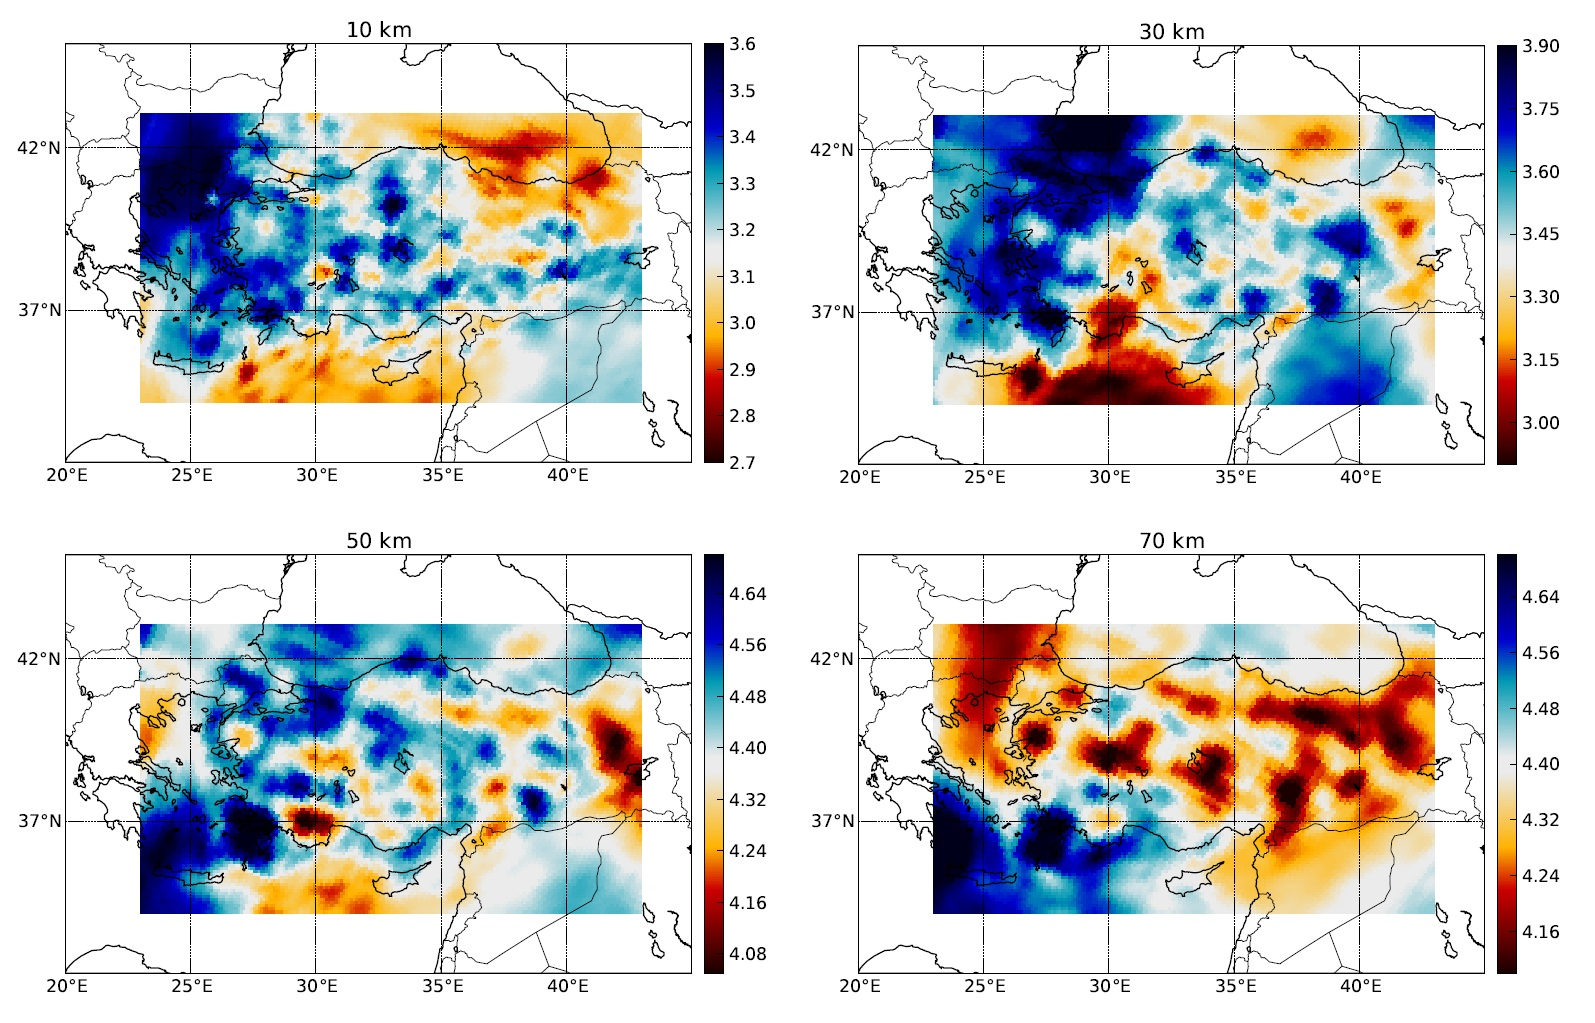
\includegraphics{Figures/anatolia.jpg}} 
\caption{Distribution of $\vsv$ in the Anatolian model at $20$ km, $50$ km and $100$ km depth. The depth slices in this figure were generated using the Python tool \texttt{models.py} in the \texttt{TOOLS} directory.}\label{F:anatolia}
\end{figure}
\end{center}
%====================================================================

%====================================================================
% Output
%====================================================================

\subsection{Simulation of wave propagation and output}

The actual wave propagation executable is \texttt{ses3d.exe}, located in \texttt{MAIN}. Upon running \texttt{ses3d.exe}, the geometrical information in \texttt{setup}, the event information in \texttt{event\_x} and \texttt{event\_list}, as well as the physical model parameters in \texttt{MODELS/MODELS} are read. The seismic wavefield is the propagated forward in time, for \texttt{nt} time steps. After the last time step, synthetic seismograms are written to the output directory, in our case \texttt{DATA/OUTPUT/1.8s/}. The three-component synthetic seismograms for station BALB are shown in figure \ref{F:seismograms}.
%====================================================================
\begin{center}
\begin{figure}
\center\scalebox{0.47}{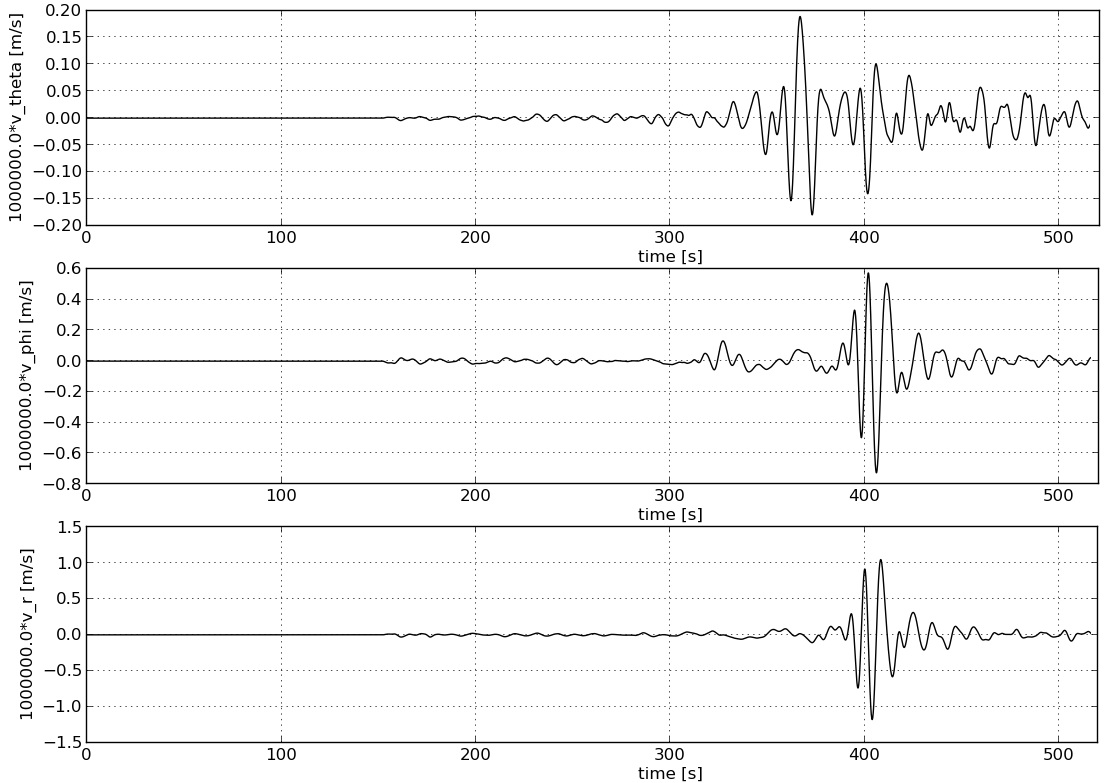
\includegraphics{Figures/seismograms.jpg}} 
\caption{Three-component synthetic seismograms for station BALB.}\label{F:seismograms}
\end{figure}
\end{center}
%====================================================================

%====================================================================
% Computing sensitivity kernels
%====================================================================

\subsection{Computing sensitivity kernels}\label{S:kernels}

The computation of sensitivity kernels proceeds in several steps. First of all, a forward simulation must be run with the \texttt{adjoint\_flag} in the \texttt{setup} file set to \texttt{1}. This ensures that the forward field is stored in the directory which appears in the last line of the \texttt{setup} file. Make sure enough storage is actually available.\\
Once the forward field is computed, adjoint sources for a variety of measurements can be computed using Python tools in the \texttt{TOOLS} directory. An example of this procedure is given below:\\[5pt]
\texttt{run seismograms.py}: Compile Python tool for reading and plotting seismograms.\\[5pt]
\texttt{run adjoint\_source.py}: Compile Python tool for the computation of adjoint sources.\\[5pt]
\texttt{s=ses3d\_seismogram()}: Make empty seismogram structure.\\[5pt]
\texttt{s.read('../DATA/OUTPUT/1.8s/','BALB\_.KO.\_\_\_')}: Read seismograms for station BALB.\\[5pt]
\texttt{s.plot(1e6)}: Plot seismograms, scaled by a factor of $1\cdot 10^6$.\\[5pt]
\texttt{a=adjoint\_source()}: Make empty adjoint source structure.\\[5pt]
\texttt{a.fetch\_seismogram(s)}: Load seismograms into the adjoint source structure.\\[5pt]
\texttt{a.make\_adsrc\_mttime('z',391.0,412.0,0.1,True)}: Compute adjoint source for a multitaper measurement of a time delay on the vertical component for the window from $391.0$ s to $412.0$ s at the frequency of $0.1$ Hz.\\[5pt]
\texttt{a.plot()}: Plot adjoint source.\\[5pt]
\texttt{a.write('../ADJOINT/1/','ad\_src\_1')}: Write adjoint source to file.\\[5pt]
It is important that the adjoint sources for \texttt{event\_1} are written to the directory \texttt{ADJOINT/1/}. For an event with event file \texttt{event\_102}, the adjoint sources would be expected to be located in \texttt{ADJOINT/102/}.\\
For each event, multiple adjoint sources may be computed. In our example, we use only one. The second adjoint source time function would be named \texttt{ad\_src\_2}, and it would be located in the same directory. The file \texttt{ad\_srcfile} contains a list of all adjoint source time functions used for this specific event. In our case, \texttt{ad\_srcfile} contains only 2 lines:\\[7pt]
\texttt{1} (indicates that one adjoint source is used)\\
\texttt{50.36 27.88 1000.0} (colatitude, longitude and depth of the adjoint source)\\[7pt]
Once the adjoint sources are computed, simply set the \texttt{adjoint\_flag} to \texttt{2} and re-run the wave propagation code. Sensitivity kernels will then be computed automatically, and stored in the output directory specified in the event file. Then, using \texttt{project\_kernels.exe} in the \texttt{TOOLS} directory, the kernels can be projected onto the grid used to represent 3D models. This is particularly helpful in the context of tomographic inverse problems, but also for plotting purposes. Since the projected kernels have the same format as a 3D model, we can use the Python tool \texttt{models.py} to read and plot the projected kernels. The result is shown in figure \ref{F:kernel}.
%====================================================================
\begin{center}
\begin{figure}
\center\scalebox{0.35}{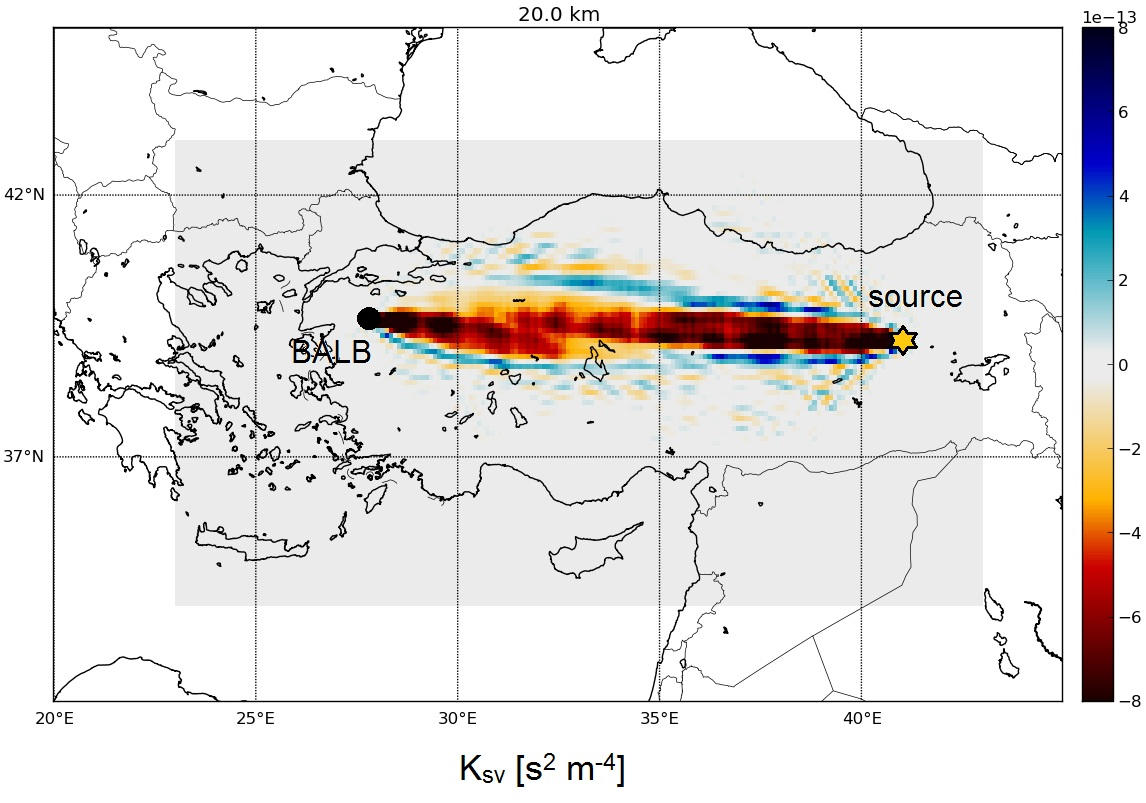
\includegraphics{Figures/kernel.jpg}} 
\caption{Sensitivity kernel with respect to the SV velocity at $20$ km depth. The measurement is  a multitaper measurement of a time delay on the vertical component of station BALB for the window from $391.0$ s to $412.0$ s at the frequency of $0.1$ Hz.}\label{F:kernel}
\end{figure}
\end{center}
%====================================================================

%====================================================================
% North America
%====================================================================

\section{Continental-scale wave propagation: North America}\label{S:North_America}

Seismic wave propagation in \SES may become inefficient when the computational domain is too close to the poles where the elements become very small, thus enforcing a small time step. This problem is particularly relevant for large domains that approach or even include the poles. To avoid excessively small time steps, the computational domain can be rotated away from the poles towards the equator.\\[5pt]
This rotation procedure will play a central role in the following scenario where we consider seismic wave propagation across North America and the North Atlantic. The scenario-specific input and source files are located in the directory \texttt{SCENARIOS/NORTH\_AMERICA}.

%====================================================================
% Rotating the computational domain.
%====================================================================

\subsection{Rotating the computational domain}

We are interested in the computational domain shown in figure \ref{F:NA1} that covers the North American continent and the North Atlantic. Since the domain closely approaches the North pole, where elements become very small, it should ideally be rotated southwards to avoid excessively small time steps. In this example, we rotate the complete domain southwards by $30^\circ$ around an axis given in terms of the unit vector
\begin{equation}
\w{n} = \left( \begin{array}{c} \text{cos}(40^\circ) \\ \text{sin}(40^\circ) \\ 0.0 \end{array} \right)
\end{equation}
The rotated domain is shown in figure \ref{F:NA2}. In rotated coordinates, the computational domain falls between the following colatitudes and longitudes that are specified in the \texttt{setup} file: \texttt{theta\_min=45.2}, \texttt{theta\_max=114.8}, \texttt{phi\_min=-119.8}, \texttt{phi\_max=-0.2}.\\[5pt]
Since the actual computations are not performed in the true physical but in the rotated domain, various input parameters must be adapted. The input parameters include the station and event coordinates, as well as the moment tensor. Python tools for the rotation of source/receiver locations and moment tensors can be found in \texttt{TOOLS/rotation.py}. These tools are also described in section \ref{S:Python}. While the original epicentral coordinates of our event are $\theta=34.08^\circ$, $\phi=-17.80^\circ$, the rotated cooridnates are $\theta'=61.30^\circ$, $\phi'=-30.10^\circ$. Similarly the moment tensor is rotated as follows:
\begin{align}
\w{M}&=\left(\begin{array}{ccc}
M_{tt} & M_{tp} & M_{tr} \\ M_{tp} & M_{pp} & M_{pr} \\ M_{tr} & M_{pr} & M_{rr}
\end{array}\right)
=
\left(\begin{array}{ccc}
-3.794 & 1.978 & -1.145 \\ 1.977 & 4.004 & -0.514 \\ -1.145 & -0.514 & -0.211
\end{array}\right) \notag\\
\to \notag \\
\w{M'}&=\left(\begin{array}{ccc}
M'_{tt} & M'_{tp} & M'_{tr} \\ M'_{tp} & M'_{pp} & M'_{pr} \\ M'_{tr} & M'_{pr} & M'_{rr}
\end{array}\right)
=
\left(\begin{array}{ccc}
-4.220 & -0.644 & -0.935 \\ -0.644 & 4.430 & -0.838 \\ -0.935 & -0.838 & -0.211
\end{array}\right) 
\end{align}
The rotated event parameters are specified in \texttt{event\_1}.\\[5pt]
Most plotting routines for models and seismograms that are located in the \texttt{TOOLS} directory, correctly account for the rotation. All that needs to be done is to set the rotation vector and the rotation angle in the file \texttt{TOOLS/rotation\_parameters.txt}.

%====================================================================
\begin{center}
\begin{figure}
\center\scalebox{0.45}{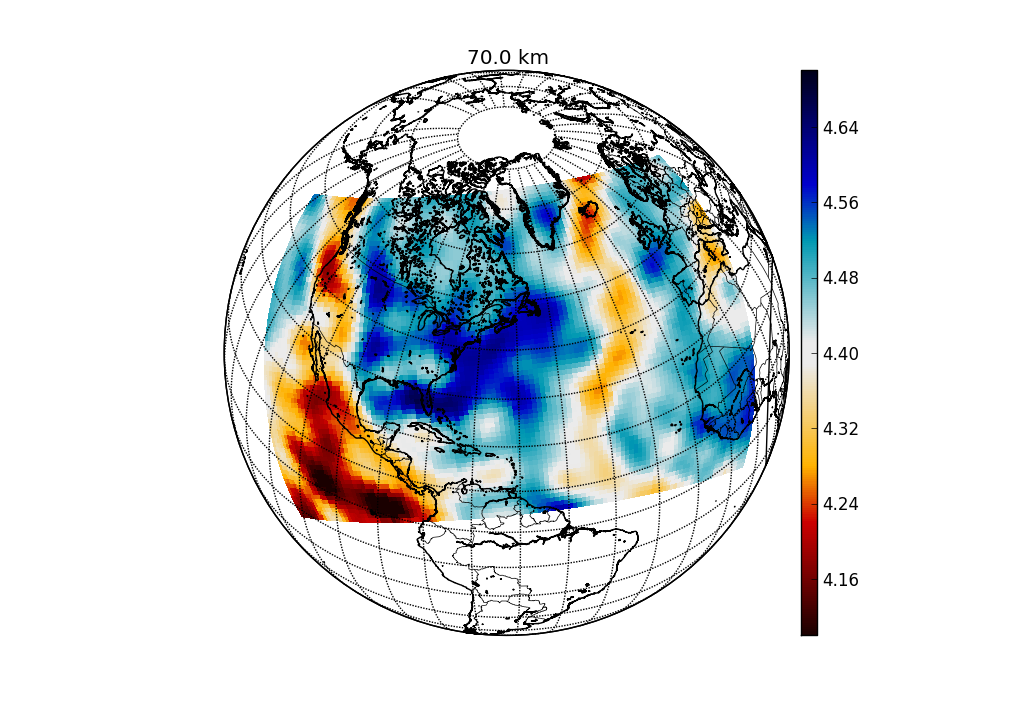
\includegraphics{Figures/NA1.png}} 
\caption{Horizontal slice through the SV velocity in model S40RTS (Ritsema et al., 2011) at $70$ km depth beneath North America and the North Atlantic. The computational domain approaches the North pole, and therefore needs to be rotated southwards. This plot was made with the tools provided in \texttt{TOOLS/models.py}.}\label{F:NA1}
\end{figure}
\end{center}
%====================================================================

%====================================================================
\begin{center}
\begin{figure}
\center\scalebox{0.45}{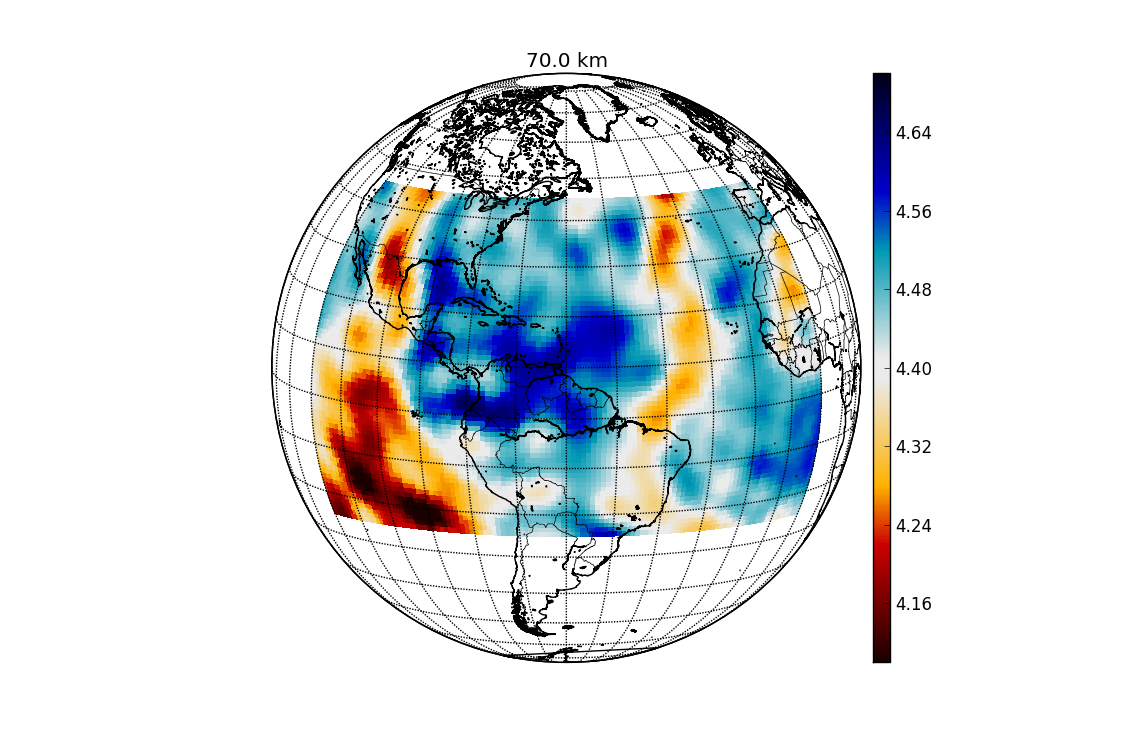
\includegraphics{Figures/NA2.png}} 
\caption{Rotated North America model. All computations are performed in this rotated domain. This plot was made with the tools provided in \texttt{TOOLS/models.py}.}\label{F:NA2}
\end{figure}
\end{center}
%====================================================================

\subsection{Source time function}\label{S:stf_NA}

While the computational domain in this scenario is comparatively large, its discretisation with $\sim 1.8$ elements per degree (specified in the \texttt{setup} file) is rather coarse. We are thus limited to the modelling of long-period wave propagation. To construct a suitable source time function, we can make use of the \texttt{make\_stf.py} scripts in the \texttt{TOOLS} directory. The function call\\[5pt]
\texttt{make\_stf(0.2,12000,1.0/200.0,1.0/100.0,'../INPUT/stf')}\\[5pt]
Produces a source time function that is a bandpass-filtered Heaviside function with cutoffs at $1/200$ Hz and $1/100$ Hz. The time step is equal to $0.2$ s, identical to the time step \texttt{dt} specified in the \texttt{setup} file. The number of time steps is $12000$, and the output file is written to \texttt{../INPUT/stf}. The source time function in the time and frequency domain is displayed in figure \ref{F:stf_NA}.
%====================================================================
\begin{center}
\begin{figure}
\center\scalebox{0.30}{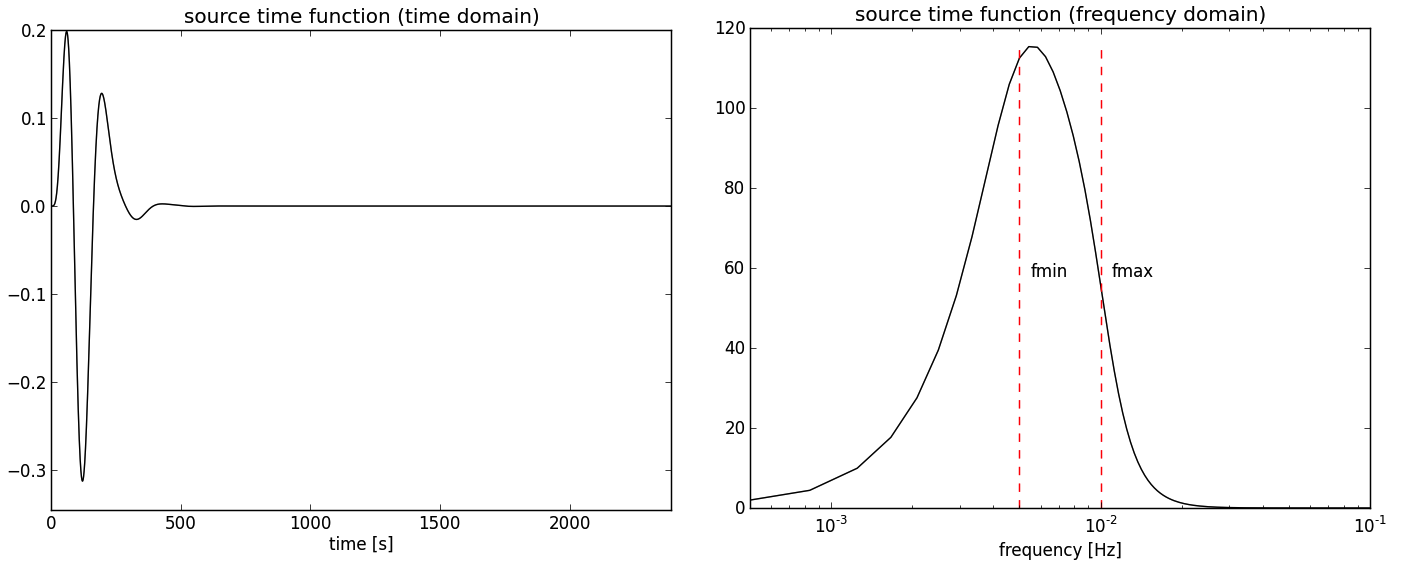
\includegraphics{Figures/stf_NA.png}} 
\caption{Time- and frequency-domain representation of the source time function produced by \texttt{make\_stf(0.2,12000,1.0/200.0,1.0/100.0,'../INPUT/stf')}}\label{F:stf_NA}
\end{figure}
\end{center}
%====================================================================

%====================================================================
% Constructing the 3D model.
%====================================================================

\subsection{Constructing the 3D model}

The construction of a 3D Earth model for this scenario is similar to the previous one described in section \ref{S:Anatolia}. The only difference is that the coordinates in the \texttt{block\_x}, \texttt{block\_y} and \texttt{block\_z} files must of course be rotated towards the equator.\\[5pt]
In the first step, we again generate a 1D model using \texttt{generate\_models}. As 1D model we choose one where all elastic parameters are set to zero, and where a smoothed version of the Q model QL6 (Durek \& Ekstr\"{o}m, 1996) is implemented. To use this model, set \texttt{model\_type} to \texttt{3} in the \texttt{setup} file. More details on visco-elastic dissipation for this specific scenario and from a more mathematical perspective can be found in sections \ref{S:NAQ} and \ref{S:attenuation}, respectively.\\[5pt] 
Following this initial step, we add 3D heterogeneities, again using \texttt{add\_perturbation}. To ensure that the heterogeneities are properly implemented, we can visualise the material parameters on the spectral-element grid using thy Python tool \texttt{ses3d\_fields.py} in the \texttt{TOOLS} directory (see also section \ref{S:Python}). The resulting plot is shown in figure \ref{F:fields}.  
%====================================================================
\begin{center}
\begin{figure}
\center\scalebox{0.3}{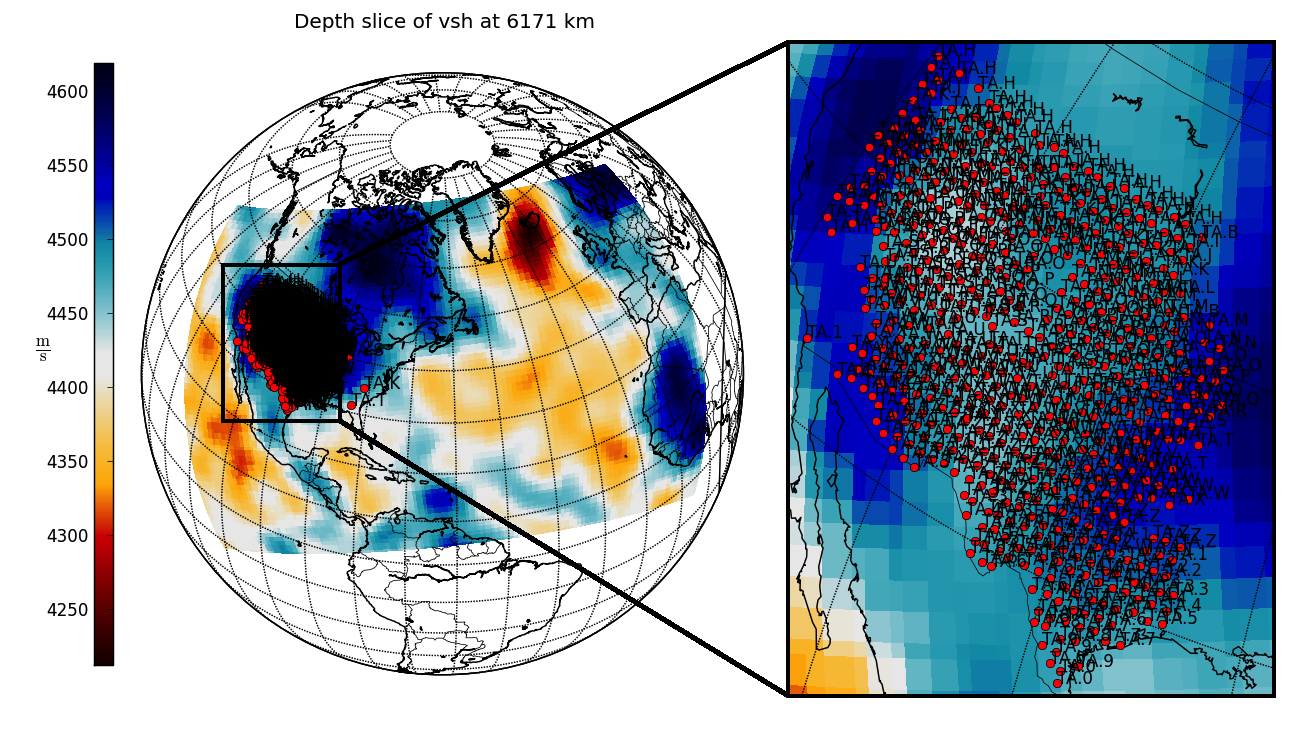
\includegraphics{Figures/fields.png}} 
\caption{Rotated North America model ($\vsv$) as implemented on the spectral-element grid. A zoom into the western part of USArray is shown to the right. This plot was made using \texttt{ses3d\_fields.py} from the \texttt{TOOLS} directory.}\label{F:fields}
\end{figure}
\end{center}
%====================================================================


\subsection{Visco-elastic dissipation}\label{S:NAQ}

To enable visco-elastic dissipation in \SES, the \texttt{is\_diss} flag in the \texttt{setup} file must be set to $1$. The mathematical description and numerical implementation of visco-elastic dissipation is described in chapter \ref{C:attenuation}. The visco-elastic properties of the Earth model are encoded in a set of relaxation parameters that can be computed using the Python code \texttt{Q\_discrete.py} located in the \texttt{TOOLS} directory. Requesting a constant $Q$ for periods between $80$ s and $250$ s, \texttt{Q\_discrete.py} produces the relaxation weights $1.684, 0.838, 1.357$, and the corresponding relaxation times $3.200, 17.692, 74.504$. These values must be written into the \texttt{relax} file in the \texttt{INPUT} directory. An illustration of the constant target $Q$ and the numerical approximation, as well as of the corresponding phase velocity dispersion, is provided in figure \ref{F:Q_NA}.
%====================================================================
\begin{center}
\begin{figure}
\center\scalebox{0.40}{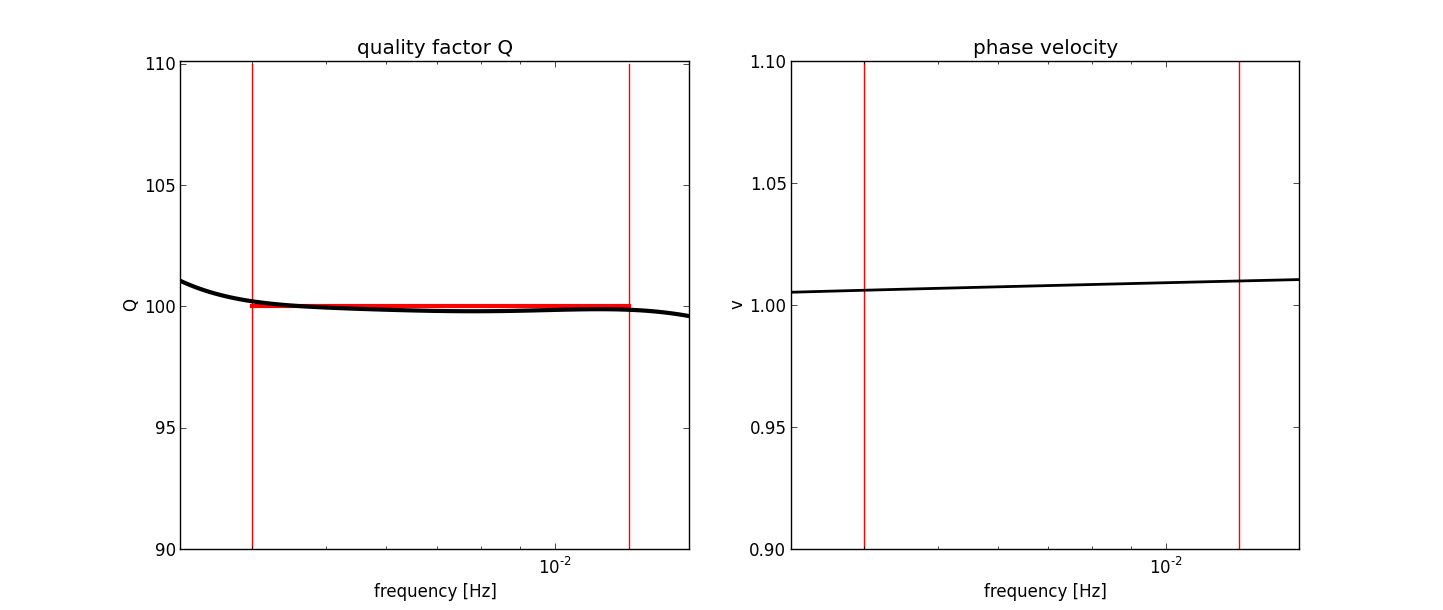
\includegraphics{Figures/Q_NA.png}} 
\caption{\textbf{Left}: Comparison of the constant target shear $Q$ with value $100$ and the corresponding numerical approximation, as computed by \texttt{Q\_discrete.py}. \textbf{Right}: Phase velocity dispersion.}\label{F:Q_NA}
\end{figure}
\end{center}
%====================================================================


\subsection{Wiggly lines}\label{S:NA_seismo}

To plot seismograms, we can use the Python class \texttt{ses3d\_seismogram} in the \texttt{TOOLS} directory. Simply run \texttt{seismograms.py} and then initiate a class member, e.g. by typing\\[5pt] 
\texttt{s=ses3d\_seismogram()}.\\[5pt] 
Using the \texttt{read} function, we can read a seismogram by giving the directory and station name:\\[5pt] \texttt{s.read('../DATA/OUTPUT/1/','TA.L16A\_.\_\_\_')}.\\[5pt]
Typing\\[5pt]
\texttt[s.plot()]\\[5pt]
will produce the plot shown in figure \ref{F:NA_seismo}. 
%====================================================================
\begin{center}
\begin{figure}
\center\scalebox{0.45}{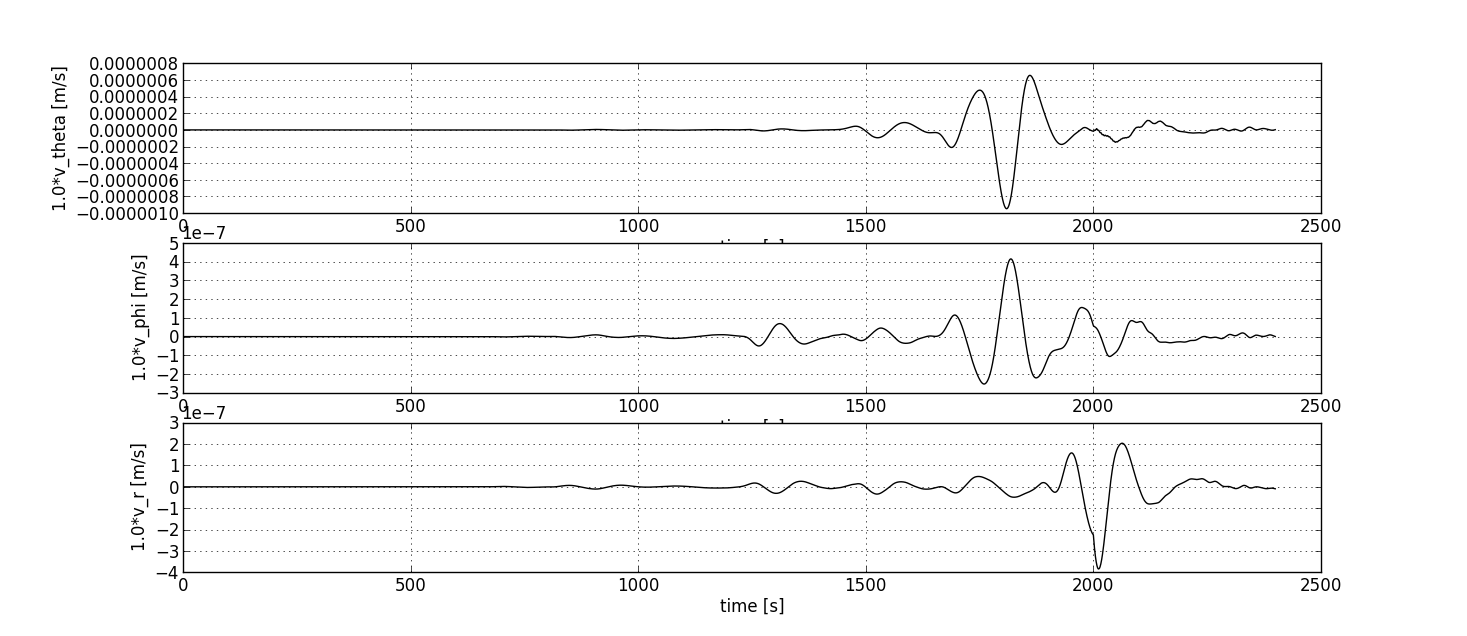
\includegraphics{Figures/seismo_example.png}} 
\caption{Three-component velocity seismograms at station TA.L16A.}\label{F:NA_seismo}
\end{figure}
\end{center}
%====================================================================